% =============================================================================
% EMBINO: Technology & Opportunity Booklet
% Grammar-Constrained Code Generation for Resource-Limited Embedded Systems
% =============================================================================

\documentclass[10pt,twoside]{report}

% =============================================================================
% PREAMBLE
% =============================================================================

% ---------- Encoding & Fonts ----------
\usepackage[utf8]{inputenc}
\usepackage[T1]{fontenc}
\usepackage{lmodern}
\usepackage{microtype}

% ---------- Page Layout ----------
\usepackage[
    papersize={6in,9in},
    margin=0.65in,
    inner=0.8in,
    outer=0.5in
]{geometry}
\usepackage{setspace}
\setstretch{1.15}

% ---------- Math ----------
\usepackage{amsmath,amssymb,amsthm}
\usepackage{mathtools}
\usepackage{bm}

% ---------- Graphics & Plotting ----------
\usepackage{tikz}
\usepackage{pgfplots}
\pgfplotsset{compat=1.18}
\usetikzlibrary{
    arrows.meta,
    positioning,
    shapes.geometric,
    shapes.misc,
    calc,
    decorations.pathreplacing,
    patterns,
    backgrounds,
    fit,
    matrix,
    chains,
    shadows
}

% ---------- Colored Boxes (auto-sizing) ----------
\usepackage[most]{tcolorbox}

% ---------- Tables & Lists ----------
\usepackage{booktabs}
\usepackage{multirow}
\usepackage{enumitem}
\usepackage{tabularx}
\setlist{nosep, leftmargin=*}

% ---------- Colors ----------
\usepackage{xcolor}
\definecolor{embinoblue}{RGB}{30,90,160}
\definecolor{embinoteal}{RGB}{0,128,128}
\definecolor{embinodark}{RGB}{25,35,55}
\definecolor{embinogold}{RGB}{218,165,32}
\definecolor{lightgray}{RGB}{245,245,245}
\definecolor{darkgray}{RGB}{64,64,64}
\definecolor{accentred}{RGB}{192,0,48}
\definecolor{codegreen}{RGB}{0,128,0}

% ---------- Code Listings ----------
\usepackage{listings}
\lstset{
    basicstyle=\ttfamily\footnotesize,
    keywordstyle=\color{embinoblue}\bfseries,
    commentstyle=\color{codegreen}\itshape,
    stringstyle=\color{embinogold},
    backgroundcolor=\color{lightgray},
    frame=single,
    framerule=0pt,
    breaklines=true,
    captionpos=b,
    numbers=left,
    numberstyle=\tiny\color{darkgray},
    tabsize=2
}

% ---------- Headers & Footers ----------
\usepackage{fancyhdr}
\pagestyle{fancy}
\fancyhf{}
\fancyhead[LE]{\footnotesize\textsc{Embino}}
\fancyhead[RO]{\footnotesize\textsc{\leftmark}}
\fancyfoot[C]{\small\thepage}
\renewcommand{\headrulewidth}{0.4pt}

% ---------- Chapter Styling ----------
\usepackage{titlesec}
\titleformat{\chapter}[display]
    {\normalfont\Large\bfseries\color{embinodark}}
    {\chaptertitlename\ \thechapter}{15pt}{\LARGE}
\titlespacing*{\chapter}{0pt}{-15pt}{20pt}

\titleformat{\section}{\normalfont\large\bfseries\color{embinodark}}{\thesection}{1em}{}
\titleformat{\subsection}{\normalfont\normalsize\bfseries}{\thesubsection}{1em}{}

% ---------- References ----------
\usepackage[hidelinks]{hyperref}
\hypersetup{
    colorlinks=true,
    linkcolor=embinoblue,
    urlcolor=embinoteal,
    citecolor=embinoblue
}
\usepackage{cleveref}

% ---------- Custom Commands ----------
\newcommand{\embino}{\textsc{Embino}}
\newcommand{\gcslm}{\textsc{GC-SLM}}
\newcommand{\slora}{\textsc{S-LoRA}}
\newcommand{\Oh}{\mathcal{O}}
\newcommand{\vocab}{\mathcal{V}}
\newcommand{\grammar}{\mathcal{G}}

% ---------- Custom Box Styles ----------
\newtcolorbox{highlightbox}[1][embinoblue]{
    colback=#1!5,
    colframe=#1,
    boxrule=1.5pt,
    arc=3pt,
    left=6pt, right=6pt, top=6pt, bottom=6pt,
    fontupper=\small
}

\newtcolorbox{phasebox}[1][embinoteal]{
    colback=#1!8,
    colframe=#1,
    boxrule=1pt,
    arc=3pt,
    left=6pt, right=6pt, top=6pt, bottom=6pt,
    fontupper=\small
}

% =============================================================================
% DOCUMENT
% =============================================================================

\begin{document}

% =============================================================================
% TITLE PAGE
% =============================================================================

\begin{titlepage}
\begin{tikzpicture}[remember picture, overlay]
    % Background gradient
    \fill[embinodark] (current page.south west) rectangle (current page.north east);
    
    % Decorative circuit pattern
    \begin{scope}[shift={(current page.center)}, opacity=0.1]
        \foreach \x in {-4,-2,0,2,4} {
            \foreach \y in {-5,-3,-1,1,3,5} {
                \draw[white, thick] (\x,\y) -- (\x+0.5,\y) -- (\x+0.5,\y+0.5);
                \fill[white] (\x,\y) circle (2pt);
            }
        }
    \end{scope}
    
    % Main content
    \node[anchor=center] at (current page.center) {
        \begin{minipage}{0.8\textwidth}
            \centering
            
            % Logo/Title
            \textcolor{embinoteal}{\rule{2cm}{2pt}}\\[0.5cm]
            {\fontsize{42}{46}\selectfont\bfseries\textcolor{white}{EMBINO}}\\[0.3cm]
            \textcolor{embinoteal}{\rule{2cm}{2pt}}\\[1.2cm]
            
            % Subtitle
            {\large\textcolor{white}{Grammar-Constrained Code Generation}}\\[0.2cm]
            {\large\textcolor{white}{for Resource-Limited Embedded Systems}}\\[1.5cm]
            
            % Tagline
            {\normalsize\textcolor{embinogold}{\textit{Tiny Intelligence for Tiny Devices}}}\\[2.5cm]
            
            % Document type
            {\small\textcolor{white!70}{Technology \& Opportunity Overview}}\\[0.2cm]
            {\small\textcolor{white!70}{Academic Research $\cdot$ Intellectual Property $\cdot$ Commercial Strategy}}\\[1.5cm]
            
            % Author/Company
            {\footnotesize\textcolor{white!50}{Kernel Keys LLC}}\\
            {\footnotesize\textcolor{white!50}{2025}}
            
        \end{minipage}
    };
\end{tikzpicture}
\end{titlepage}

% =============================================================================
% COPYRIGHT PAGE
% =============================================================================

\thispagestyle{empty}
\vspace*{\fill}
\begin{center}
    \small
    \textcopyright\ 2025 Kernel Keys LLC. All rights reserved.\\[0.8cm]
    
    \textbf{Provisional Patent Application Filed}\\
    \textit{Systems and Methods for Grammar-Constrained Code Generation}\\
    \textit{and Execution on Resource-Limited Embedded Devices}\\[0.8cm]
    
    \textbf{Contact}\\
    david@kernelkeys.com\\
    www.kernelkeys.com\\[1.5cm]
    
    {\footnotesize\textcolor{darkgray}{This document contains confidential information.\\
    Distribution without authorization is prohibited.}}
\end{center}
\vspace*{\fill}
\clearpage

% =============================================================================
% TABLE OF CONTENTS
% =============================================================================

\tableofcontents
\clearpage

% =============================================================================
% EXECUTIVE SUMMARY
% =============================================================================

\chapter*{Executive Summary}
\addcontentsline{toc}{chapter}{Executive Summary}
\markboth{Executive Summary}{}

\begin{highlightbox}
\textbf{The Opportunity}\\[0.15cm]
\embino{} bridges the gap between human intent and embedded implementation. Using small language models with grammar-constrained decoding, we enable natural-language programming of microcontrollers---without the resource requirements of large language models.
\end{highlightbox}

\section*{The Problem}

Microcontrollers power 30--40 billion devices annually, yet programming them remains stuck in 1985: hand-written C/C++, manual memory management, device-specific registers, and zero abstraction for intent.

\section*{Our Solution}

\embino{} provides a complete stack:
\begin{itemize}
    \item \textbf{\gcslm{} Framework:} Transformers under 50M params with grammar-guided decoding ensuring 100\% syntactic validity
    \item \textbf{Domain-Specific Language:} Expressive rule-based constructs for embedded control
    \item \textbf{Micro-Interpreter:} Deterministic bytecode execution in under 16KB RAM
\end{itemize}

\section*{Intellectual Property}

Provisional patent filed: 35 claims across 5 independent inventions.

\section*{Key Metrics}

\begin{center}
\footnotesize
\begin{tabular}{lccc}
\toprule
\textbf{Metric} & \textbf{LLM} & \textbf{MicroPython} & \textbf{\embino{}} \\
\midrule
Model size & 1--175B & N/A & 1--50M \\
RAM required & 8--128GB & 256KB+ & $<$16KB \\
Syntax validity & 70--90\% & N/A & 100\% \\
MCU deployment & No & Limited & Yes \\
\bottomrule
\end{tabular}
\end{center}

\clearpage

% =============================================================================
% CHAPTER 1: TECHNOLOGY OVERVIEW
% =============================================================================

\chapter{Technology Overview}
\label{ch:technology}

\section{The Abstraction Gap}

The history of programming abstraction is one of steady ascent: machine code gave way to assembly; assembly to C; C to higher-level languages. Yet embedded systems remain stuck at C/C++.

Large language models demonstrate code generation capabilities, but their size (billions of parameters) and latency render them unsuitable for microcontrollers with kilobytes of memory.

\embino{} addresses this gap.

\begin{figure}[h]
\centering
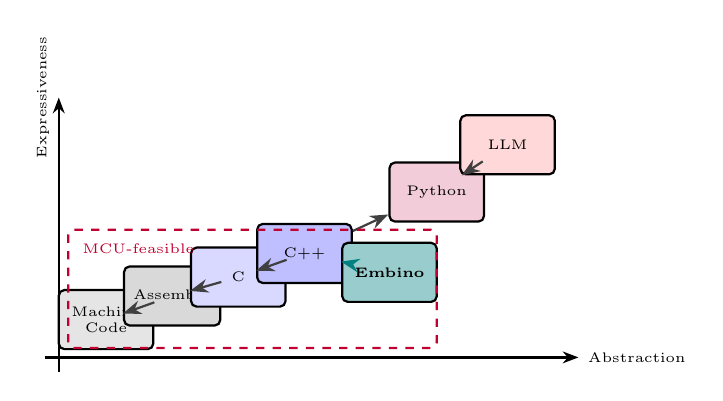
\begin{tikzpicture}[
    x=0.6cm, y=0.6cm,
    era/.style={
        rectangle, rounded corners=2pt,
        minimum width=1.2cm, minimum height=0.75cm,
        draw, thick, align=center, font=\tiny
    }
]

% Axes
\draw[thick, -{Stealth[length=2mm]}] (-0.3,0) -- (11,0);
\draw[thick, -{Stealth[length=2mm]}] (0,-0.3) -- (0,5.5);
\node[font=\tiny, anchor=west] at (11,0) {Abstraction};
\node[font=\tiny, anchor=south, rotate=90] at (0,5.5) {Expressiveness};

% Eras
\node[era, fill=gray!20] (mc)  at (1, 0.8) {Machine\\Code};
\node[era, fill=gray!30] (asm) at (2.4, 1.3) {Assembly};
\node[era, fill=blue!15] (c)   at (3.8, 1.7) {C};
\node[era, fill=blue!25] (cpp) at (5.2, 2.2) {C++};
\node[era, fill=embinoteal!40, thick] (slm) at (7, 1.8) {\textbf{\embino{}}};
\node[era, fill=purple!20] (py)  at (8, 3.5) {Python};
\node[era, fill=red!15] (llm) at (9.5, 4.5) {LLM};

% Arrows
\draw[-{Stealth}, thick, darkgray] (mc) -- (asm);
\draw[-{Stealth}, thick, darkgray] (asm) -- (c);
\draw[-{Stealth}, thick, darkgray] (c) -- (cpp);
\draw[-{Stealth}, thick, darkgray] (cpp) -- (py);
\draw[-{Stealth}, thick, darkgray] (py) -- (llm);
\draw[-{Stealth}, thick, embinoteal, dashed] (cpp) -- (slm);

% MCU-feasible region
\draw[thick, dashed, accentred, rounded corners=2pt] (0.2, 0.2) rectangle (8, 2.7);
\node[font=\tiny, accentred, anchor=north west] at (0.3, 2.6) {MCU-feasible};

\end{tikzpicture}
\caption{Evolution of programming abstraction. \embino{} occupies the upper-right of the MCU-feasible region.}
\label{fig:timeline}
\end{figure}

\section{Grammar-Constrained Small Language Models}

The \gcslm{} framework combines three innovations:

\subsection{Small Language Models}

Transformer models in the 1--50M parameter range:

\begin{center}
\footnotesize
\begin{tabular}{lccc}
\toprule
\textbf{Size} & \textbf{Layers} & \textbf{Hidden} & \textbf{Params} \\
\midrule
Tiny & 4 & 256 & 4M \\
Small & 6 & 384 & 15M \\
Base & 8 & 512 & 45M \\
\bottomrule
\end{tabular}
\end{center}

\subsection{Grammar-Guided Decoding}

At each generation step, the decoder: (1) computes logits, (2) queries parser for valid continuations, (3) masks invalid tokens, (4) samples from constrained distribution. This guarantees 100\% syntactic validity.

\subsection{Search Space Reduction}

For a typical DSL with $k \approx 50$ valid tokens per state and vocabulary $|\vocab| = 32{,}000$:
\[
\text{Reduction} = \left(\frac{|\vocab|}{k}\right)^L = 640^L
\]
For a 50-token program: $640^{50} \approx 10^{140}$ reduction.

\section{Sparse Low-Rank Adaptation (S-LoRA)}

Standard LoRA introduces adapters $\Delta W = AB$. \slora{} adds structured sparsity:
$\Delta W = (A \odot M_A)(B \odot M_B)$
where $M_A, M_B$ are binary masks.

\textbf{Benefits:} 60\% fewer adapter parameters, compatible with 8-bit quantization.

\section{Micro-Interpreter}

\begin{center}
\footnotesize
\begin{tabular}{ll}
\toprule
\textbf{Property} & \textbf{Specification} \\
\midrule
Program memory & $<$16 KB \\
Data memory & $<$4 KB \\
Stack depth & 32 elements (fixed) \\
Memory allocation & None (static only) \\
\bottomrule
\end{tabular}
\end{center}

\clearpage

% =============================================================================
% CHAPTER 2: INTELLECTUAL PROPERTY
% =============================================================================

\chapter{Intellectual Property}
\label{ch:ip}

\section{Patent Overview}

A provisional patent application has been filed covering the core innovations.

\begin{highlightbox}
\textbf{Title:} Systems and Methods for Grammar-Constrained Code Generation and Execution on Resource-Limited Embedded Devices

\vspace{0.2cm}
\textbf{Claims:} 35 total (5 independent, 30 dependent)

\vspace{0.1cm}
\textbf{Status:} Provisional application filed
\end{highlightbox}

\section{Independent Claims}

The patent covers five independent inventions:

\begin{enumerate}
    \item \textbf{Generation System:} GC-SLM + grammar decoder + compiler + micro-interpreter
    \item \textbf{Programming Method:} NL $\rightarrow$ DSL $\rightarrow$ bytecode $\rightarrow$ MCU execution
    \item \textbf{Embedded Apparatus:} MCU with interpreter, fixed stack, hardware interfaces
    \item \textbf{Decoding Method:} Grammar-constrained token generation
    \item \textbf{Adaptation System:} S-LoRA with sparse low-rank matrices
\end{enumerate}

\section{Key Dependent Claims}

\begin{center}
\footnotesize
\begin{tabular}{cp{6.5cm}}
\toprule
\textbf{Claim} & \textbf{Coverage} \\
\midrule
6--7 & Model size ($<$50M, $<$10M quantized) \\
8 & MCU targets (ESP32, RP2040, ATmega, STM32) \\
9--10 & Memory constraints, no dynamic allocation \\
26--30 & S-LoRA specifics (masks, sparsity, quantization) \\
31--32 & On-device generation, FPGA implementation \\
\bottomrule
\end{tabular}
\end{center}

\section{Freedom to Operate}

The invention occupies a novel intersection of three domains:

\begin{figure}[h]
\centering
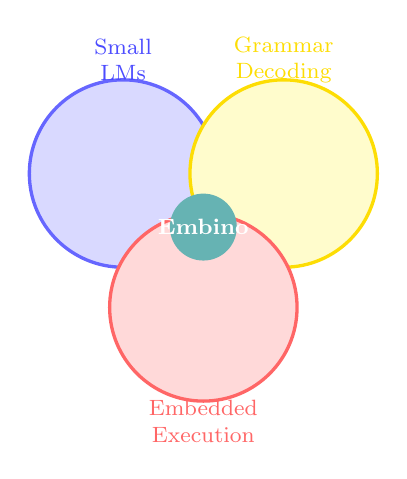
\begin{tikzpicture}[scale=0.85]
    % Three separate circles with clear boundaries
    \draw[very thick, blue!60, fill=blue!15] (-1.2,0.8) circle (1.4cm);
    \draw[very thick, yellow!80!orange, fill=yellow!20] (1.2,0.8) circle (1.4cm);
    \draw[very thick, red!60, fill=red!15] (0,-1.2) circle (1.4cm);
    
    % Labels outside circles
    \node[font=\footnotesize, align=center, blue!70] at (-1.2,2.5) {Small\\LMs};
    \node[font=\footnotesize, align=center, yellow!80!orange] at (1.2,2.5) {Grammar\\Decoding};
    \node[font=\footnotesize, align=center, red!60] at (0,-2.9) {Embedded\\Execution};
    
    % Center intersection highlight
    \fill[embinoteal!60] (0,0) circle (0.5cm);
    \node[font=\footnotesize\bfseries, white] at (0,0) {\embino{}};
    
\end{tikzpicture}
\caption{Patent coverage at the intersection of three domains.}
\end{figure}

Prior art addresses individual components but not the integrated system.

\clearpage

% =============================================================================
% CHAPTER 3: COMMERCIAL OPPORTUNITY
% =============================================================================

\chapter{Commercial Opportunity}
\label{ch:commercial}

\section{Market Landscape}

\begin{center}
\footnotesize
\begin{tabular}{ll}
\toprule
\textbf{Metric} & \textbf{Value} \\
\midrule
MCU annual shipments & 30--40 billion units \\
Dev board volume & Tens of millions/year \\
Addressable (0.1\%) & 30--40 million units/year \\
\bottomrule
\end{tabular}
\end{center}

\section{The Problem We Solve}

Programming microcontrollers requires C/C++ expertise, memory management, register knowledge, timing/interrupts, and specialized debug toolchains.

\textbf{Alternatives fall short:}
\begin{itemize}
    \item \textbf{MicroPython:} 256KB+ RAM, unpredictable timing
    \item \textbf{Block programming:} Limited expressiveness, cloud-dependent
    \item \textbf{LLMs:} Cannot run on-device, produce invalid code
\end{itemize}

\section{Competitive Landscape}

\begin{center}
\footnotesize
\begin{tabular}{lcccc}
\toprule
\textbf{Solution} & \textbf{Abstraction} & \textbf{MCU-Safe} & \textbf{Deterministic} & \textbf{AI} \\
\midrule
C/C++ & Low & Yes & Yes & No \\
MicroPython & High & Partial & No & No \\
Block coding & Medium & Yes & Yes & No \\
LLM APIs & High & No & No & Yes \\
\textbf{\embino{}} & \textbf{High} & \textbf{Yes} & \textbf{Yes} & \textbf{Yes} \\
\bottomrule
\end{tabular}
\end{center}

\section{Business Model}

\begin{enumerate}
    \item \textbf{Hardware sales:} Dev boards and modules
    \item \textbf{Software licensing:} Toolchain subscriptions
    \item \textbf{Enterprise licensing:} Custom integrations
    \item \textbf{IP licensing:} Per-unit royalties for OEMs
\end{enumerate}

\clearpage

% =============================================================================
% CHAPTER 4: HARDWARE ROADMAP & FUNDING
% =============================================================================

\chapter{Hardware Roadmap \& Funding}
\label{ch:roadmap}

\section{Three-Stage Hardware Strategy}

\subsection{Stage 1: Add-On Module (12--24 months)}

\begin{phasebox}[embinoteal]
\textbf{Product:} External board via UART/I$^2$C/SPI

\textbf{Target:} Makers, educators, robotics hobbyists

\textbf{Revenue:} Dev board sales, starter kits

\textbf{Price:} \$15--35 per unit

\textbf{Advantage:} Zero changes to existing boards
\end{phasebox}

\subsection{Stage 2: System-on-PCB (24--36 months)}

\begin{phasebox}[embinoblue]
\textbf{Product:} Integrated board with \embino{} runtime

\textbf{Target:} Robotics startups, automation integrators

\textbf{Revenue:} Volume board sales, subscriptions

\textbf{Price:} \$8--20 per unit (volume)

\textbf{Advantage:} Standard Arduino/Pico pinout
\end{phasebox}

\subsection{Stage 3: On-Chip / Custom Silicon (36+ months)}

\begin{phasebox}[embinogold!80!black]
\textbf{Product:} MCU with ROM-resident interpreter

\textbf{Target:} Appliance manufacturers, industrial OEMs

\textbf{Revenue:} Licensing fees, per-unit royalties

\textbf{Price:} \$0.10--0.50 per chip (licensing)

\textbf{Advantage:} Lowest BOM, highest scale
\end{phasebox}

\clearpage

\section{Funding Requirements}

\subsection{Phase 1: Proof of Concept (\$500K, 12 months)}

\begin{phasebox}[accentred]
\textbf{Deliverables:}
\begin{itemize}
    \item DSL specification and grammar
    \item Working GC-SLM prototype (15M params)
    \item Micro-interpreter on ESP32/Arduino
    \item 3 demo applications with metrics
    \item User study with 8--10 participants
\end{itemize}
\end{phasebox}

\subsection{Phase 2: Product Development (\$2M, 18 months)}

\begin{phasebox}[embinoblue]
\textbf{Deliverables:}
\begin{itemize}
    \item Production-ready add-on module
    \item Cloud toolchain and IDE
    \item 5+ paying pilot customers
    \item Multi-MCU support (ESP32, RP2040, STM32)
    \item Patent prosecution and IP strengthening
\end{itemize}
\end{phasebox}

\subsection{Phase 3: Scale to Breakeven (\$5--6M, 24--36 months)}

\begin{phasebox}[embinoteal]
\textbf{Deliverables:}
\begin{itemize}
    \item System-on-PCB product line
    \item Enterprise licensing agreements
    \item 50+ enterprise customers
    \item Custom silicon partnerships
    \item Path to profitability / breakeven
\end{itemize}
\end{phasebox}

\section{Funding Summary}

\begin{center}
\begin{tabular}{llcl}
\toprule
\textbf{Phase} & \textbf{Funding} & \textbf{Timeline} & \textbf{Milestone} \\
\midrule
1. PoC & \$500K & 12 mo & Working prototype \\
2. Product & \$2M & +18 mo & Paying customers \\
3. Scale & \$5--6M & +24--36 mo & Breakeven company \\
\midrule
\textbf{Total} & \textbf{\$7.5--8.5M} & \textbf{4--5 years} & \\
\bottomrule
\end{tabular}
\end{center}

\section{Use of Funds}

\begin{center}
\footnotesize
\begin{tabular}{lrrr}
\toprule
\textbf{Category} & \textbf{Phase 1} & \textbf{Phase 2} & \textbf{Phase 3} \\
\midrule
Engineering (R\&D) & 60\% & 50\% & 35\% \\
Hardware/Prototypes & 15\% & 20\% & 25\% \\
Operations & 15\% & 15\% & 20\% \\
Sales/Marketing & 5\% & 10\% & 15\% \\
Legal/IP & 5\% & 5\% & 5\% \\
\bottomrule
\end{tabular}
\end{center}

\clearpage

% =============================================================================
% CHAPTER 5: TECHNICAL SPECIFICATIONS
% =============================================================================

\chapter{Technical Specifications}
\label{ch:specs}

\section{System Requirements}

\subsection{Generation System (Edge/Cloud)}

\begin{center}
\footnotesize
\begin{tabular}{ll}
\toprule
\textbf{Component} & \textbf{Requirement} \\
\midrule
Model size & 4M--45M parameters \\
Inference hardware & CPU (x86/ARM), GPU optional \\
RAM & 256MB--2GB \\
Latency & $<$500ms per program \\
Syntax validity & 100\% (guaranteed) \\
\bottomrule
\end{tabular}
\end{center}

\subsection{Target Hardware}

\begin{center}
\footnotesize
\begin{tabular}{lccc}
\toprule
\textbf{MCU} & \textbf{Flash} & \textbf{RAM} & \textbf{Clock} \\
\midrule
ESP32 & 4MB & 520KB & 240MHz \\
RP2040 & 2MB & 264KB & 133MHz \\
ATmega328 & 32KB & 2KB & 16MHz \\
STM32F4 & 512KB & 128KB & 168MHz \\
\bottomrule
\end{tabular}
\end{center}

\section{DSL Grammar (Excerpt)}

\begin{lstlisting}[language=Python, caption={DSL grammar (BNF)}]
program     ::= statement+
statement   ::= assignment | conditional | loop | action
conditional ::= 'when' condition ':' action+
loop        ::= 'every' duration ':' action+
action      ::= 'set' target 'to' value | 'wait' duration
\end{lstlisting}

\section{Bytecode Instruction Set}

\begin{center}
\footnotesize
\begin{tabular}{llc}
\toprule
\textbf{Opcode} & \textbf{Description} & \textbf{Bytes} \\
\midrule
\texttt{PUSH/POP} & Stack operations & 1--5 \\
\texttt{LOAD/STORE} & Variable access & 2 \\
\texttt{READ\_SENSOR} & Sensor input & 2 \\
\texttt{SET\_PIN} & GPIO output & 3 \\
\texttt{JUMP/JUMP\_IF} & Control flow & 3 \\
\texttt{WAIT/HALT} & Timing/termination & 1--3 \\
\bottomrule
\end{tabular}
\end{center}

\section{Safety Guarantees}

\begin{enumerate}
    \item \textbf{Syntactic validity:} Grammar constraints ensure valid programs
    \item \textbf{Resource bounds:} Static analysis verifies memory/stack
    \item \textbf{Timing bounds:} WCET analysis for real-time guarantees
    \item \textbf{Pin safety:} Configurable write protection
\end{enumerate}

\clearpage

% =============================================================================
% CHAPTER 6: THEORETICAL FOUNDATIONS
% =============================================================================

\chapter{Theoretical Foundations}
\label{ch:theory}

\section{Complexity Analysis}

\begin{highlightbox}[darkgray]
\textbf{Proposition (Decoding Complexity).}
Grammar-guided decoding adds $\Oh(|G| + |\vocab|)$ time per token.
\end{highlightbox}

For typical DSLs ($|G| \approx 100$, $|\vocab| \approx 32{,}000$): $<$1ms per token.

\section{Capacity Lower Bounds}

\begin{highlightbox}[darkgray]
\textbf{Theorem.} A transformer generating programs for grammar $\grammar$ with $n$ rules, depth $\ell$, and $c$ semantic classes requires:
\[|\theta| \geq \Omega\left(\frac{c \log(n\ell)}{\epsilon}\right)\]
parameters to achieve loss $< \epsilon$.
\end{highlightbox}

\textit{Implication:} For $n=50$, $\ell=10$, $c=1000$, $\epsilon=0.1$: lower bound $\approx 600$K params. Models with 1--50M are well above this.

\section{Sample Complexity}

\begin{highlightbox}[darkgray]
\textbf{Theorem.} S-LoRA fine-tuning requires 
\[N = \Oh\left(\frac{sm \cdot c}{\epsilon^2}\right)\]
training examples for $\epsilon$-accuracy.
\end{highlightbox}

For typical values: $\approx 10$K curated examples with augmentation.

\clearpage

% =============================================================================
% APPENDIX: PATENT CLAIMS SUMMARY
% =============================================================================

\appendix

\chapter{Patent Claims Reference}
\label{app:claims}

\begin{center}
\footnotesize
\begin{tabular}{cp{7cm}}
\toprule
\textbf{\#} & \textbf{Summary} \\
\midrule
1 & System: GC-SLM + grammar decoder + compiler + interpreter \\
2 & Method: NL $\rightarrow$ DSL $\rightarrow$ bytecode $\rightarrow$ MCU \\
3 & Apparatus: MCU with interpreter, fixed stack \\
4 & Decoding: Grammar-constrained token generation \\
5 & Adaptation: S-LoRA with sparse matrices \\
\midrule
6--7 & Model size constraints \\
8 & Target MCUs (ESP32, RP2040, etc.) \\
9--13 & Memory, safety, verification \\
14--20 & Decoding and training specifics \\
21--25 & Timing, scheduling, safety \\
26--30 & S-LoRA implementation details \\
31--35 & On-device, FPGA, multi-grammar \\
\bottomrule
\end{tabular}
\end{center}

\chapter{Contact Information}
\label{app:contact}

\begin{center}
\vspace{1.5cm}

{\large\textbf{Kernel Keys LLC}}\\[0.8cm]

\textbf{Primary Contact}\\
David H.\ Silver, Founder\\[0.4cm]

\textbf{Email:} david@kernelkeys.com\\[0.3cm]

\textbf{Web:} www.kernelkeys.com / www.embino.com\\[1.5cm]

\rule{4cm}{0.4pt}\\[0.8cm]

{\footnotesize\textit{For investment inquiries, partnership opportunities,\\or technical collaboration.}}

\end{center}

% =============================================================================
% END
% =============================================================================

\end{document}
